\section{Abordagens utilizadas}



\subsection{Sistemas baseados em filtros colaborativos}

Nestes sistemas são utilizadas as várias avaliações dos utilizadores para se fazerem recomendações. 

\subsubsection{Filtros colaborativos baseados em utilizadores}

Neste caso, as classificações fornecidas por utilizadores com os mesmos gostos de A são usadas para as recomendações para A.
Para este filtro foi implementado uma função que encontra pessoas que viram os mesmos filmes, retornando a um determinado utilizador a lista dos filmes vistos pelos 10 utilizadores com gostos mais semelhantes. Como esta implementação foi a combinação de duas técnicas o código será apresentado nos Sistemas Híbridos. 


\subsection{Sistemas baseados em conteúdo}

Nestes sistemas, as avaliações do utilizador, assim como os géneros de filmes que ele costuma gostar, são combinados com os atributos dos filmes para fazer as recomendações. 
Para esta abordagem, através dos géneros dos filmes que o utilizador já viu, são adicionados a uma lista dois filmes desses mesmos géneros, não repetindo filmes no caso de haver filmes com mais do que um tipo de género.

\begin{figure}[H]
\centering
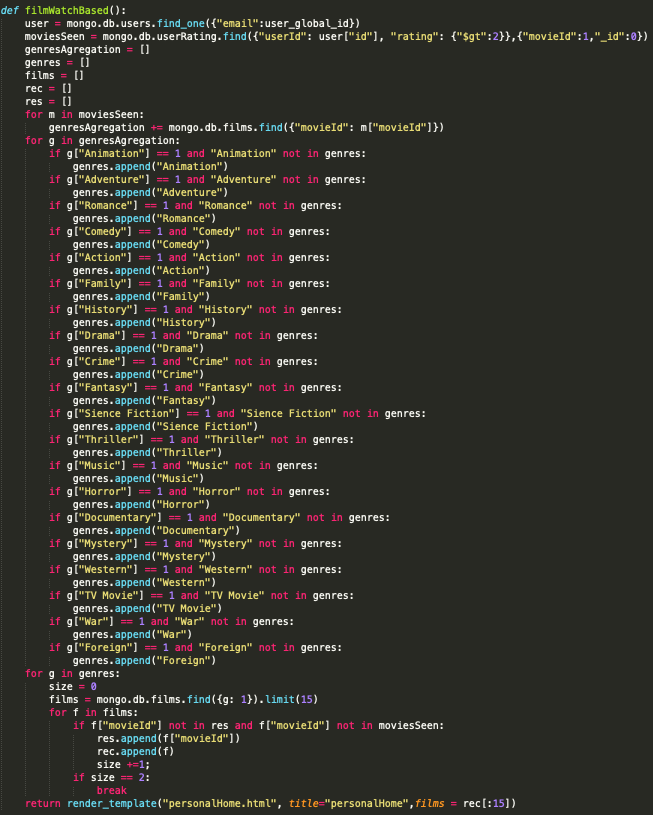
\includegraphics[scale=0.7]{content.png}
\end{figure}


\subsection{Sistemas baseado em restrições}
Neste caso através da aplicação Web o utilizador pode fazer uma pesquisa com uma determinada palavra, que tanto pode pertencer ao título, ao resumo ou até ao género do filme, e são-lhe apresentados filmes contendo essa mesma palavra

\begin{figure}[H]
\centering
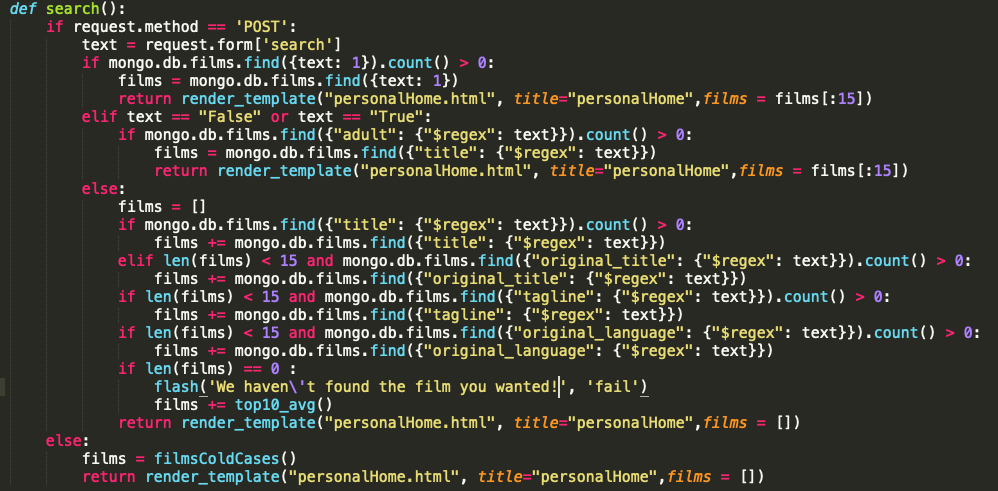
\includegraphics[scale=0.5]{restricao.png}
\end{figure}
 

\subsection{Sistemas baseados em conhecimento}

Uma das vantagens destes sistemas é que são particularmente úteis em casos em que não há histórico de filmes ou avaliações, ou cenários de \textit{cold-start}. Para este caso, foi implementada uma função que devolve os 10 filmes mais bem cotados.


\begin{figure}[H]
\centering
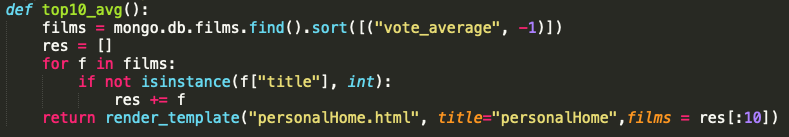
\includegraphics[scale=0.6]{coldstart.png}
\end{figure}


\subsection{Sistemas Híbridos}

A vantagem destes sistemas é que são capazes de combinar vários modelos.
Para estes sistemas utilizámos filtros colaborativos baseados em utilizadores, e nos casos de \textit{cold start} utilizámos a técnica usada nos sistemas baseados em conhecimento.

\begin{figure}[H]
\centering
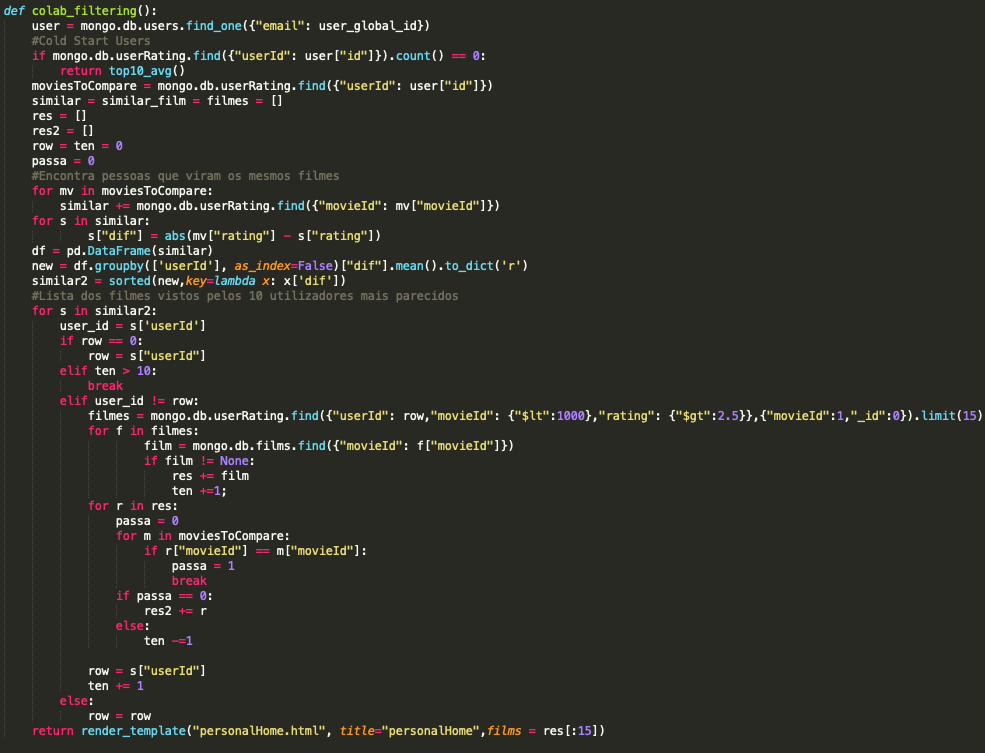
\includegraphics[scale=0.4]{colab.png}
\end{figure}



\newpage

